%%%%%%%% MiLeTS 2026 — ACM SIGKDD (sigconf) VERSION %%%%%%%%
% Content identical to main_milets2026.tex (negative-result/open-problem reframe),
% ported to acmart sigconf for SIGKDD formatting compliance.
% ⚠️ UNTESTED — produced without local TeX. Compile and fix any acmart-specific
%    errors (needs acmart.cls, standard in TeXLive/MiKTeX). natbib (\citep/\citet)
%    is on by default in acmart, so citations should resolve against references.bib.
% Blind: MiLeTS blind policy unconfirmed. If double-blind, add option `anonymous`
%    to \documentclass and the author block auto-hides. If single-blind/non-blind,
%    leave as is.
% Do NOT overwrite base main.tex or paper/submissions/{SPIGM,FMSD}/.

% CAMERA-READY (MiLeTS 2026, accepted 2026-06-14). De-anonymized: the `anonymous`
% option is removed so the author block below is shown. The submission version used
% [sigconf,nonacm,anonymous] for the double-blind review round.
\documentclass[sigconf,nonacm]{acmart}

\usepackage{graphicx}
\usepackage{booktabs}
\usepackage{amsmath}
\let\Bbbk\relax % avoid clash: acmart/newtxmath already defines \Bbbk
\usepackage{amssymb}

\microtypesetup{expansion=true,protrusion=true} % fonts now properly mapped (scalable); enable for tight justification
\setlength{\emergencystretch}{2em} % last-resort stretch to clear margin overflows in narrow 2-col
\settopmatter{printacmref=false} % no ACM reference block (workshop, non-archival)
\setcopyright{none}
\renewcommand\footnotetextcopyrightpermission[1]{}

\begin{document}

\title{When Does Adversarial Refinement Help? A Negative Result and Open Problem in Adapting R3GAN to Time Series Imputation}

\author{Yufeng He}
\affiliation{%
  \institution{The University of Hong Kong}
  \city{Hong Kong}
  \country{China}}
\email{he-yufeng@connect.hku.hk}

\begin{abstract}
Diffusion models and transformers have supplanted GANs for multivariate time series imputation, largely on grounds of GAN training instability.
R3GAN (NeurIPS 2024) removes that instability via regularized relativistic losses with provable convergence, raising a natural question: do stable, modern GANs revive adversarial imputation?
We adapt R3GAN to 1D temporal data with a coarse-to-fine refinement framework and a frequency-domain discriminator, and run a systematic study across 3 datasets and 15+ configurations.
\textbf{We report a negative result.}
R3GAN-1D refinement dramatically improves \emph{distributionally implausible} coarse imputers (48--70\% MAE reduction over mean/zero fill) but yields no improvement over a \emph{strong} coarse imputer (linear interpolation, $|\Delta|<1.5\%$), and as a standalone imputer it underperforms BRITS by $5.8\times$.
Crucially, we argue the common explanation---that GANs optimize distributional rather than point-wise objectives---\emph{cannot} be the whole story, since diffusion models also optimize distributional objectives yet achieve state-of-the-art imputation.
Our ablations instead implicate the \emph{adversarial signal specifically}: increasing the reconstruction weight (suppressing the adversarial term) never hurts accuracy, suggesting the gains come from supervised reconstruction rather than the discriminator (a controlled discriminator-removed ablation, our key next experiment, would confirm this).
We frame the precise reason a learned discriminator fails to provide useful refinement gradients---where a learned diffusion denoiser succeeds---as an open problem, and offer practical guidance on when adversarial refinement is worthwhile.
\end{abstract}

\keywords{time series imputation, GAN, R3GAN, adversarial refinement, negative result}

\maketitle

\section{Introduction}

Missing values are ubiquitous in multivariate time series (MTS) from domains including healthcare, environmental monitoring, and industrial systems.
Accurate imputation is critical, as missing data degrades the performance of downstream tasks such as forecasting and anomaly detection.

The imputation landscape has evolved rapidly.
RNN-based approaches like BRITS~\citep{cao2018brits} model bidirectional temporal dynamics.
Transformer-based methods such as SAITS~\citep{du2023saits} leverage self-attention for long-range dependencies.
More recently, diffusion models like CSDI~\citep{tashiro2021csdi} and FGTI~\citep{wang2024fgti} achieve state-of-the-art through iterative denoising.
GAN-based imputation, pioneered by GRUI-GAN~\citep{luo2018grui} and GAIN~\citep{yoon2018gain}, showed early promise but has largely vanished from top venues since 2019. The IJCAI 2025 survey~\citep{wang2025survey} notes that GANs ``may face convergence difficulties that can affect imputation accuracy.''

R3GAN~\citep{huang2024r3gan}, a modern GAN with regularized relativistic loss and R1/R2 gradient penalties, achieves provable local convergence for image generation without normalization layers. This makes it a clean testbed for a question the field has not revisited since GANs fell out of favour: \textit{once training instability is removed, can a modern GAN improve time series imputation?}

Our answer is \textbf{largely no}, and we think the negative result is more informative than another marginal positive would have been. We make three contributions:
(1)~\textbf{R3GAN-1D}, a faithful 1D adaptation of R3GAN with a frequency-domain discriminator branch, trained \emph{stably} across all our runs (so instability is no longer a confound);
(2)~a \textbf{systematic refinement study} across 3 datasets and 15+ configurations that isolates exactly where adversarial refinement helps (trivial coarse imputers) and where it does not (strong coarse imputers, and standalone use);
(3)~an \textbf{honest diagnosis and open problem}: the textbook ``distributional-vs-point-wise'' explanation is internally inconsistent (diffusion is also distributional, yet SoTA), our ablations point to the adversarial signal specifically, and we articulate what a correct explanation must account for.

\section{Related Work}

\textbf{Time series imputation.}
Classical methods include mean/median fill and linear interpolation.
Deep learning approaches span RNN-based (BRITS~\citep{cao2018brits}), attention-based (SAITS~\citep{du2023saits}, ImputeFormer~\citep{nie2024imputeformer}), and generative models.
Among generative approaches, diffusion models (CSDI~\citep{tashiro2021csdi}, FGTI~\citep{wang2024fgti}) now dominate, while GAN-based methods (GRUI-GAN~\citep{luo2018grui}, GAIN~\citep{yoon2018gain}, SSGAN~\citep{miao2021ssgan}) have declined due to training instability.
TSI-Bench~\citep{bansal2024tsibench} provides a comprehensive benchmark showing no single method dominates across all settings.
That diffusion models---also generative, also distribution-matching---now lead imputation is central to our diagnosis (\S\ref{sec:analysis}): it rules out ``generative/distributional objective'' as a blanket explanation for GAN failure.

\textbf{R3GAN.}
\citet{huang2024r3gan} propose a minimalist GAN framework using relativistic paired loss (RpGAN) with zero-centered R1 and R2 gradient penalties. Combined with ResNet-style generators using Fixup initialization (eliminating all normalization layers), R3GAN achieves competitive image generation quality with provable local convergence. Our work is the first to adapt R3GAN to temporal data, and we use its stability precisely to remove instability as an explanation for poor imputation.

\textbf{Coarse-to-fine imputation.}
Two-stage approaches have been explored in image inpainting, where a coarse network provides initial structure and a refinement network adds detail. We adapt this paradigm to time series, using any simple imputer as the coarse stage and R3GAN as the refinement stage.

\section{Method}

\subsection{R3GAN-1D Architecture}

We adapt R3GAN from 2D image generation to 1D time series, replacing all Conv2d operations with Conv1d and 2D interpolative resampling with 1D lowpass-filtered interpolation using a $[1,2,1]$ kernel.

\textbf{Generator.}
A U-Net-style encoder-decoder with skip connections. Each stage contains inverted-bottleneck residual blocks with grouped convolutions and Fixup initialization (no batch/layer/instance normalization). The generator takes as input the concatenation $[\mathbf{X}_{\text{obs}}, \mathbf{M}, \mathbf{X}_c, \mathbf{z}]$ along the feature dimension, where $\mathbf{X}_{\text{obs}}$ is observed data, $\mathbf{M}$ is the binary observation mask ($M_{tf}=1$ at observed positions and $0$ at missing positions), $\mathbf{X}_c$ is the coarse imputation, and $\mathbf{z} \sim \mathcal{N}(0, I)$ is noise. It outputs a residual $\Delta$:
\begin{equation}
    \hat{\mathbf{X}} = \mathbf{X}_{\text{obs}} \odot \mathbf{M} + (\mathbf{X}_c + \Delta) \odot (1 - \mathbf{M})
\end{equation}
This residual design ensures observed values are preserved exactly and reduces the learning burden---the generator only needs to learn corrections to the coarse estimate.

\textbf{Discriminator.}
Processes complete time series through residual blocks with progressive downsampling. We add a \textbf{frequency-domain branch}: the input's FFT magnitude spectrum is processed by a parallel path, and both features are concatenated before the final logit. This encourages the generator to match spectral characteristics of real data.

\subsection{Training Objective}

Following R3GAN~\citep{huang2024r3gan}, the discriminator uses the regularized relativistic paired loss:
\begin{equation}
    \mathcal{L}_D = \mathbb{E}[\text{sp}(-(D(\mathbf{x}_r) - D(\hat{\mathbf{x}})))] + \frac{\gamma}{2}(R_1 + R_2)
\end{equation}
where $\text{sp}(\cdot) = \log(1 + e^{(\cdot)})$ is the softplus function, and $R_1 = \mathbb{E}[\|\nabla D(\mathbf{x}_r)\|^2]$, $R_2 = \mathbb{E}[\|\nabla D(\hat{\mathbf{x}})\|^2]$ are zero-centered gradient penalties on real and fake samples respectively.

The generator loss combines three terms:
\begin{equation}
    \mathcal{L}_G = \mathcal{L}_{\text{adv}} + \lambda_r \mathcal{L}_{\text{rec}} + \lambda_f \mathcal{L}_{\text{freq}}
\end{equation}
where $\mathcal{M} = \{(t,f) : M_{tf}=0\}$ is the set of \emph{missing} positions (the complement of the observation mask $\mathbf{M}$), $\mathcal{L}_{\text{rec}} = \frac{1}{|\mathcal{M}|}\sum_{(t,f) \in \mathcal{M}} |\hat{x}_{tf} - x_{tf}|$ is the L1 reconstruction loss computed only over those missing positions, and $\mathcal{L}_{\text{freq}} = \||\text{FFT}(\hat{\mathbf{X}})| - |\text{FFT}(\mathbf{X})|\|_1$ encourages spectral fidelity.

We apply cosine learning rate decay, Adam optimizer with $\beta_1 = 0$, $\beta_2 = 0.9$, and maintain an exponential moving average (EMA) of generator weights for evaluation.

\section{Experiments}

\textbf{Datasets.}
We evaluate on three benchmarks spanning different domains and scales: \textbf{Weather} (52K timesteps, 21 meteorological features), \textbf{Electricity} (140K timesteps, 370 client consumption features), and \textbf{AirQuality} (8.7K timesteps, 36 PM2.5 monitoring stations, with 13\% original missing values).

\textbf{Protocol.}
We apply 25\% artificial point-missing (MCAR) and use a 70/15/15 train/val/test split with StandardScaler normalization. Metrics are computed only on artificially masked positions.

\textbf{R3GAN-1D configuration.}
Width=64, 3 stages, 2 blocks/stage, cardinality=16, noise dimension=32. Training: lr=$10^{-4}$, $\gamma$=0.5, $\lambda_r$=20, $\lambda_f$=2, batch size=32, cosine LR decay, EMA. Early stopping based on validation MAE.

\textbf{Baselines.}
BRITS~\citep{cao2018brits} and SAITS~\citep{du2023saits} via the PyPOTS toolkit, plus standard coarse methods (zero fill, mean fill, linear interpolation).

\subsection{Refinement Effectiveness}

\begin{table}[t]
\centering
\caption{R3GAN-1D refinement results (MAE$\downarrow$). $\Delta$: relative MAE reduction (positive = improvement). Large gains appear only when the coarse imputer is distributionally implausible (mean/zero fill); refining a strong coarse imputer (linear interpolation) yields no improvement.}
\label{tab:refinement}
\small
\begin{tabular}{@{}llccc@{}}
\toprule
Dataset & Coarse Method & Before & After & $\Delta$ \\
\midrule
Weather & Zero fill & 0.728 & 0.228 & \textbf{+68.6\%} \\
        & Mean fill & 0.728 & 0.223 & \textbf{+69.4\%} \\
        & Linear interp & 0.067 & 0.067 & +1.1\% \\
\midrule
Electricity & Zero fill & 0.832 & 0.426 & \textbf{+48.7\%} \\
            & Mean fill & 0.831 & 0.429 & \textbf{+48.4\%} \\
            & Linear interp & 0.164 & 0.165 & $-$0.7\% \\
\midrule
AirQuality & Zero fill & 0.765 & 0.228 & \textbf{+70.2\%} \\
           & Linear interp & 0.151 & 0.152 & $-$0.4\% \\
\bottomrule
\end{tabular}
\end{table}

Table~\ref{tab:refinement} reveals a striking and consistent pattern across all three datasets: R3GAN-1D provides dramatic improvement when refining weak coarse imputations (48--70\% MAE reduction from mean/zero fill) but negligible or slightly negative change when refining strong ones ($|\Delta| < 1.5\%$ for linear interpolation). Figure~\ref{fig:refinement} visualizes this asymmetry. We stress that the large percentages are improvements over \emph{trivial} baselines and should not be read as competitive performance (cf.\ Table~\ref{tab:sota}).

\begin{figure}[t]
\centering
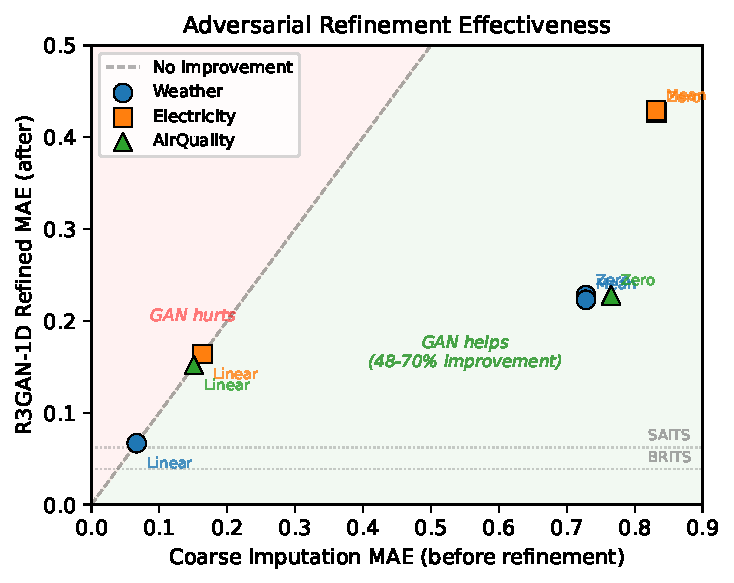
\includegraphics[width=0.85\columnwidth]{figures/refinement_plot.pdf}
\caption{Refined MAE vs.\ coarse MAE across all experiments. Points far below the diagonal indicate large improvement. Weak coarse methods (right side) benefit dramatically from GAN refinement, while strong ones (left side) see no benefit. Dashed horizontal lines mark BRITS/SAITS baselines.}
\label{fig:refinement}
\end{figure}

\subsection{Comparison with Established Methods}

\begin{table}[t]
\centering
\caption{Comparison on Weather (rate=0.25, point missing). R3GAN-1D does not match supervised baselines or even linear interpolation.}
\label{tab:sota}
\small
\begin{tabular}{@{}llcc@{}}
\toprule
Method & Type & MAE$\downarrow$ & MSE$\downarrow$ \\
\midrule
BRITS~\citep{cao2018brits} & RNN & \textbf{0.039} & \textbf{0.028} \\
SAITS~\citep{du2023saits} & Transformer & 0.062 & 0.031 \\
Linear interpolation & Simple & 0.067 & 0.079 \\
R3GAN-1D + linear & GAN refine & 0.067 & 0.076 \\
R3GAN-1D standalone & GAN & 0.228 & 0.226 \\
\bottomrule
\end{tabular}
\end{table}

Table~\ref{tab:sota} shows that R3GAN-1D as a standalone imputer (MAE=0.228) is 5.8$\times$ worse than BRITS (0.039). Refining linear interpolation leaves it statistically unchanged (0.067 $\to$ 0.067), still behind SAITS (0.062). \textbf{The honest summary is that R3GAN-1D never improves on a competent baseline}; its only ``wins'' are over baselines (mean/zero fill) that no practitioner would deploy.

\subsection{Ablation Studies}

\textbf{Data augmentation.}
Temporal flip and Gaussian jitter---standard augmentations in image GANs---consistently degrade imputation quality ($-$1.8\% to $-$3.0\% across datasets). Time series have inherent directional temporal dynamics that are destroyed by flipping, unlike the approximate spatial symmetry in natural images.

\textbf{Reconstruction weight $\lambda_r$ (key ablation).}
We sweep $\lambda_r \in \{20, 50, 100\}$. Lower values let the adversarial loss dominate and inject distributional noise that \emph{increases} point-wise error; higher values suppress the adversarial signal but \emph{do not} reduce accuracy below what the coarse method already provides. In other words, across this sweep the adversarial term is at best inert and at worst harmful for point-wise accuracy---the supervised reconstruction term carries the useful signal. We return to this in \S\ref{sec:analysis}. Short of a full recon-only ablation (Limitations), this is the closest evidence we have, and on it the discriminator does not appear to be the source of any point-wise gain; we report this as what the current evidence suggests rather than as a settled conclusion.

\textbf{Frequency-domain discriminator.}
The FFT branch provides marginal benefit (+0.25\% on Weather), suggesting that for this task, the time-domain signal already contains sufficient information for the discriminator.

\section{Analysis: Why, and What Remains Open}
\label{sec:analysis}

\textbf{Why does refinement help weak coarse imputers?}
Mean and zero fill produce outputs that are distributionally implausible---constant or zero stretches where temporal variation should exist.
Transforming these into distributionally realistic signals requires matching global statistics (variance, autocorrelation, spectral density) rather than predicting exact values, which is what an adversarial objective rewards. Hence the large gains in Table~\ref{tab:refinement}---but only relative to baselines that are already far from the data manifold.

\textbf{Why does it fail on strong coarse imputers?}
Linear interpolation already produces locally smooth, temporally coherent signals that sit close to the real-data manifold.
Further improvement requires \emph{point-wise} corrections---the exact deviation from the interpolated value at each missing position.
Empirically (the $\lambda_r$ ablation), the adversarial term supplies no useful gradient for such corrections and can inject ``creative'' variation that raises point-wise error while preserving distributional plausibility.

\textbf{What the usual explanation gets wrong.}
It is tempting to conclude a ``fundamental tension'' between distributional optimization (GANs) and point-wise metrics (MAE/MSE). \emph{We caution against this explanation.}
Diffusion models such as CSDI and FGTI also optimize a distributional/generative objective, yet are state-of-the-art on exactly these point-wise metrics. A blanket ``distributional objectives can't do point-wise imputation'' claim is therefore falsified by existing results. Whatever explains R3GAN-1D's failure must be specific to \emph{adversarial} training, not to generative modelling in general.

\textbf{An open problem.}
We can only sharpen, not settle, the question. A working hypothesis: a diffusion model is trained by a per-position denoising regression conditioned on observed values, so its learning signal is itself point-wise and observation-aware; a GAN discriminator instead scores \emph{global} plausibility and, once the input is already on-manifold, backpropagates little position-specific information. If correct, the deficit is in the \emph{form of the learning signal} (global discrimination vs.\ conditional per-position regression), not in distribution-matching per se. Testing this---e.g., by replacing the discriminator with a conditional, per-position critic, or by interpolating between adversarial and denoising-score objectives---is, to our knowledge, open. We offer R3GAN-1D and this framing as a concrete starting point.

\textbf{Practical guidance.}
From our experiments we recommend:
(1) for accuracy-critical imputation, prefer supervised or diffusion methods (BRITS, SAITS, CSDI);
(2) treat GANs as \emph{coarse reconstructors} only when starting from trivial baselines, or as data augmenters generating plausible synthetic samples;
(3) hybrid designs---e.g., GAN-generated augmentation to improve a supervised or diffusion imputer---may combine distributional diversity with point-wise precision, but this remains to be demonstrated.

\section{Limitations}

Our study is deliberately scoped and has clear limitations.
First, we report point-missing (MCAR) at a single 25\% rate on three datasets with single training seeds; block-missing, higher rates, and multi-seed error bars may shift the picture, though the qualitative asymmetry is stable across the three datasets we tried.
Second, and most important, \textbf{we do not include a full recon-only (discriminator-removed) ablation}; our evidence that the adversarial signal is not the source of any gain is indirect, via the $\lambda_r$ sweep. A controlled recon-only run is the single most valuable next experiment and we expect it to confirm the diagnosis.
Third, our supervised comparison (Table~\ref{tab:sota}) is reported on Weather, and the diffusion methods central to our argument (CSDI, FGTI) are cited rather than re-run in our protocol; an in-protocol diffusion baseline across all three datasets is the natural complement to the recon-only ablation, and we leave both to follow-up work.
Fourth, we evaluate reconstruction MAE/MSE only, not downstream-task utility; a distributionally richer imputer could in principle help downstream tasks even at equal MAE.
We flag these so the negative result is read for exactly what it supports: within stable, modern adversarial refinement at this scope, the discriminator does not deliver point-wise gains over a competent coarse imputer.

\section{Conclusion}

We adapted R3GAN to time series imputation, removing training instability as a confound, and report a negative result: stable, modern adversarial refinement helps only distributionally trivial coarse imputers and never matches supervised or diffusion baselines.
We argue the popular ``distributional-vs-point-wise'' explanation cannot be right---diffusion is also distributional yet SoTA---and our ablations instead implicate the adversarial signal specifically, leaving the precise mechanism as an open problem with a concrete hypothesis to test.
We hope a clearly-scoped negative result, with the confounder of instability controlled, saves others the same experiment and points the open question in a more productive direction than ``GANs just don't work here.''

\textbf{Code:} available from the author on request.

\bibliographystyle{ACM-Reference-Format}
\bibliography{references}

\end{document}
